\documentclass{beamer}
\usepackage[fontsize=20pt]{fontsize}
\usepackage{graphicx}
\usepackage{tikz}
\usepackage{svg}
\usepackage[polish]{babel}
\graphicspath{ {./images/} }
\usetheme{Warsaw}

%Information to be included in the title page:

% Custom title page layout adjustments
\title{\large Porównanie wydajności i możliwości współczesnych silników do gier komputerowych}
\author{Krzysztof Rudnicki}
\institute{
    \textbf{Promotor} \\
    dr inż. Michał Chwesiuk
}
\date{\scriptsize \today} % Adjust the font size here


\setbeamertemplate{footline}[frame number]{}
\beamertemplatenavigationsymbolsempty
\setbeamertemplate{headline}{}






\begin{document}

\begin{frame}
  \vspace{-0.5cm} % Adjust vertical space above title
  \maketitle
  % Alternatively, use a completely custom layout:
  %\begin{center}
  %    {\Large\inserttitle\par}
  %    \vskip1em
  %    {\insertauthor\par}
  %    \vskip1em
  %    {\insertinstitute\par}
  %    \vskip1em
  %    {\insertdate\par}
  %\end{center}
\end{frame}

\begin{frame}
\frametitle{Plan prezentacji}
\tableofcontents
\end{frame}

\section{Definicje}
\begin{frame}
  \frametitle{Gra komputerowa}
  \large Aplikacja dostępna na platformie "Steam" oznaczona typem "Game"
\end{frame}
\begin{frame}
\frametitle{Silnik do gier}
\large Oprogramowanie zaprojektowane i stworzone do kreacji gier komputerowych
\end{frame}

\begin{frame}
  \frametitle{Nowoczesne}
  \large Ponad 1000 gier w tej dekadzie na platformie "Steam"
\end{frame}


{
  \setbeamercolor{footline}{fg=white}
\usebackgroundtemplate{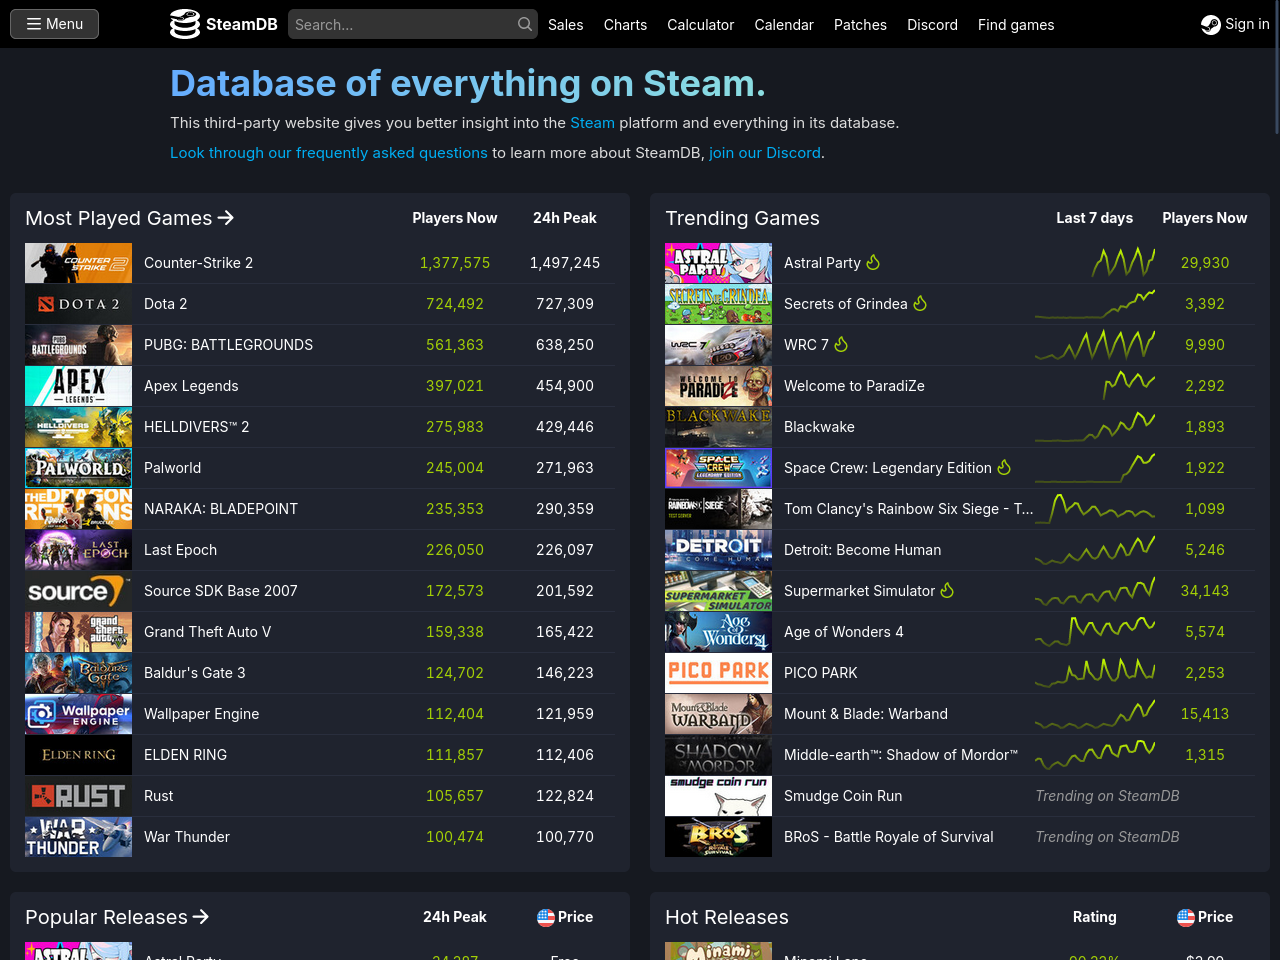
\includegraphics[width=\paperwidth, height=\paperheight]{steamdb_main.png}}
\begin{frame}
\end{frame}
}


{
\usebackgroundtemplate{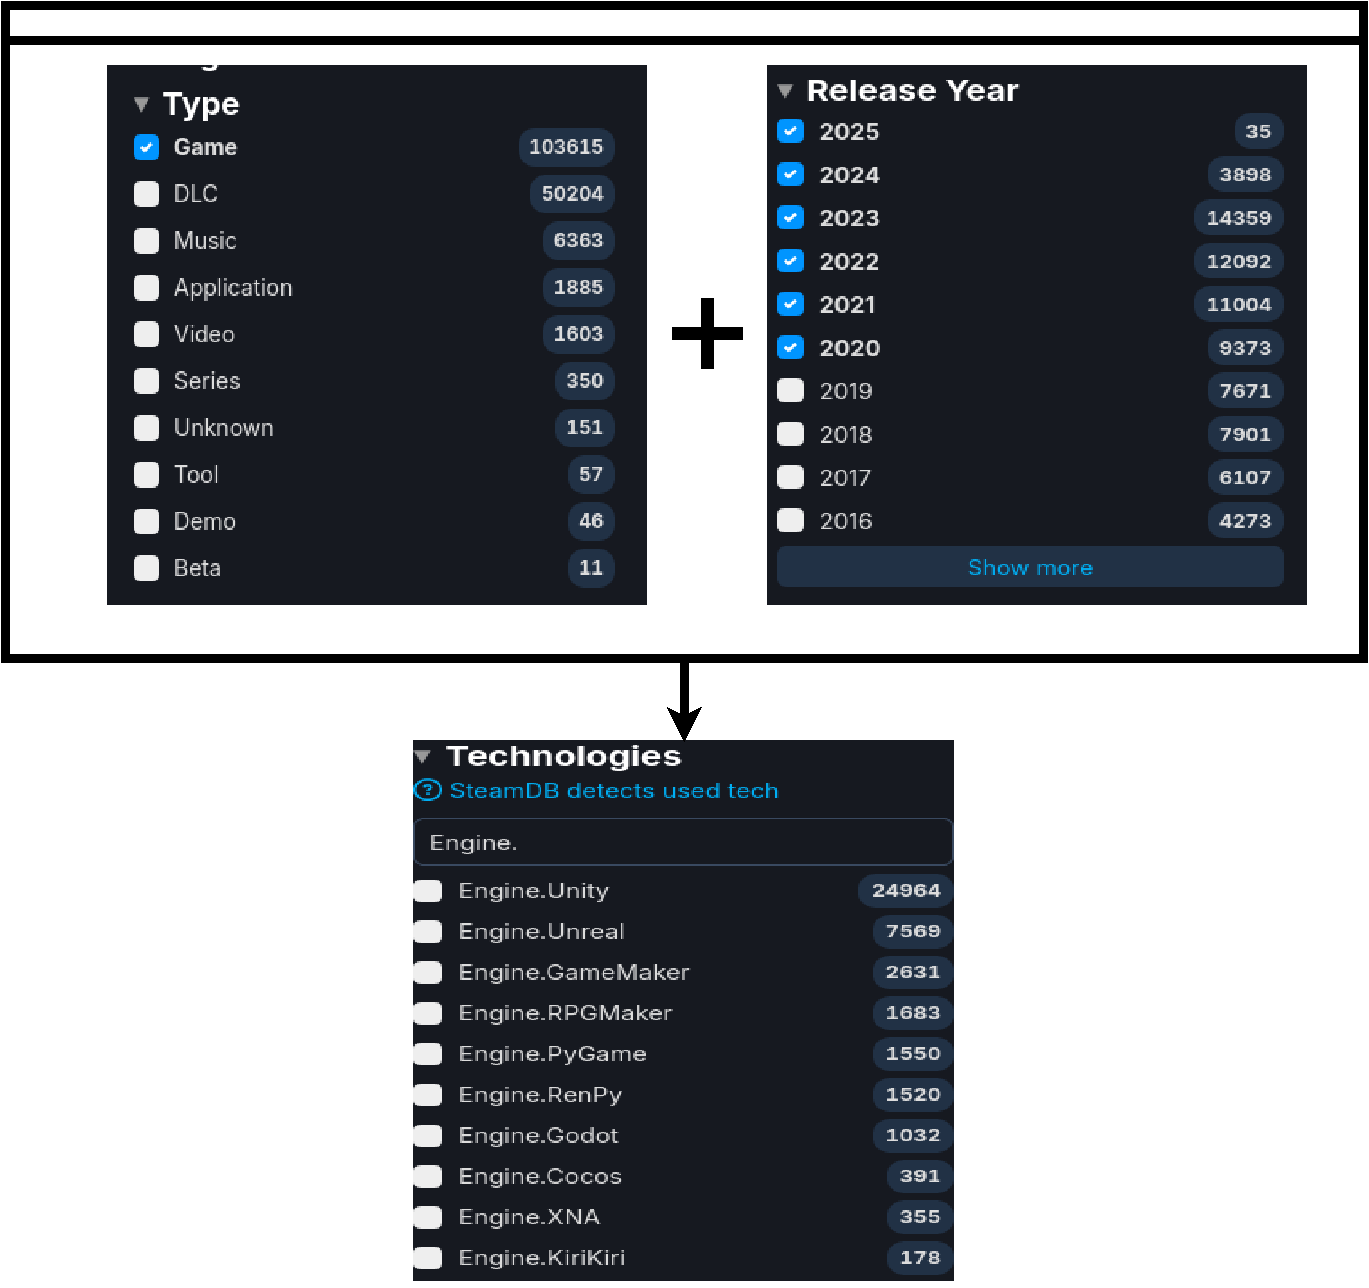
\includegraphics[width=\paperwidth, height=\paperheight]{steamdb_filter.drawio.pdf}}
\begin{frame}
\end{frame}
}

\begin{frame}
  \frametitle{Wybrane silniki - start}
  \begin{center}    
  
\includegraphics[width=0.8\paperwidth, height=0.8\paperheight]{usedEngines.pdf}
\end{center}
\end{frame}

\begin{frame}
  \frametitle{Wybrane silniki}
  \begin{itemize}
    \item Wyeliminowanie nie generycznych - Ren'Py, RPGMaker
    \item Wybór najpopularniejszych - Unity, Unreal 
    % Prawie 25k i ponad 7.5k
  \end{itemize}
\end{frame}

\begin{frame} 
  \frametitle{Wydajność silnika}
  \begin{itemize}
    \item Klatki na sekundę (FPS)
    \item Zużycie CPU, GPU, RAM i VRAM
    \item Liczba draw calls 
    \item Czas ładowania assetów 
    \item Czas odpowiedzi na interakcję gracza
  \end{itemize} 
\end{frame}
\begin{frame}
    \frametitle{Możliwości Silnika}
    \begin{itemize}
        \item Renderowanie grafiki 
        % Ray tracing, HDR lighting, dynamic shadows, particle systems, animacja
        \item Silnik Fizyczny 
        \item Multiplatformowość (VR)
        % Linux, Windows, MacOS, Android, IOs, Xbox, PlayStation, Nintendo, VR
        \item Skryptowanie logiki gier (AI)
        \item Gry online
        \item Sklepy z assetami
    \end{itemize}
  \end{frame}
    \section{Narzędzia}
      \frametitle{Unity Profiler}
      {
        \setbeamercolor{footline}{fg=white}
        \usebackgroundtemplate{
          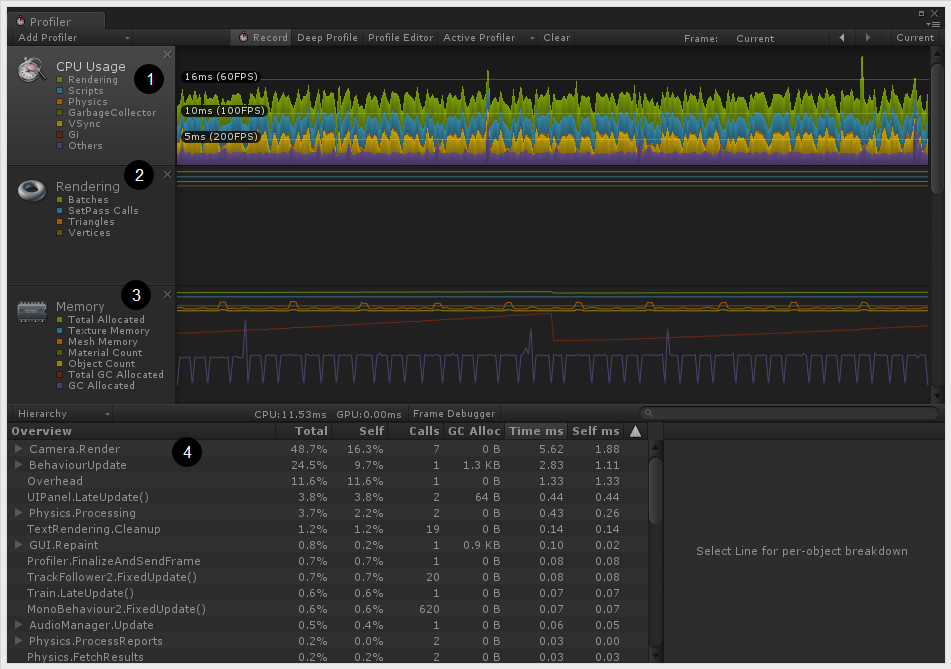
\includegraphics[width=\paperwidth, height=\paperheight]
          {unity_profiler.png}}
        \begin{frame}
        \end{frame}
        }

        \frametitle{Unreal Profiler}
        {
          \setbeamercolor{footline}{fg=white}
          \usebackgroundtemplate{
            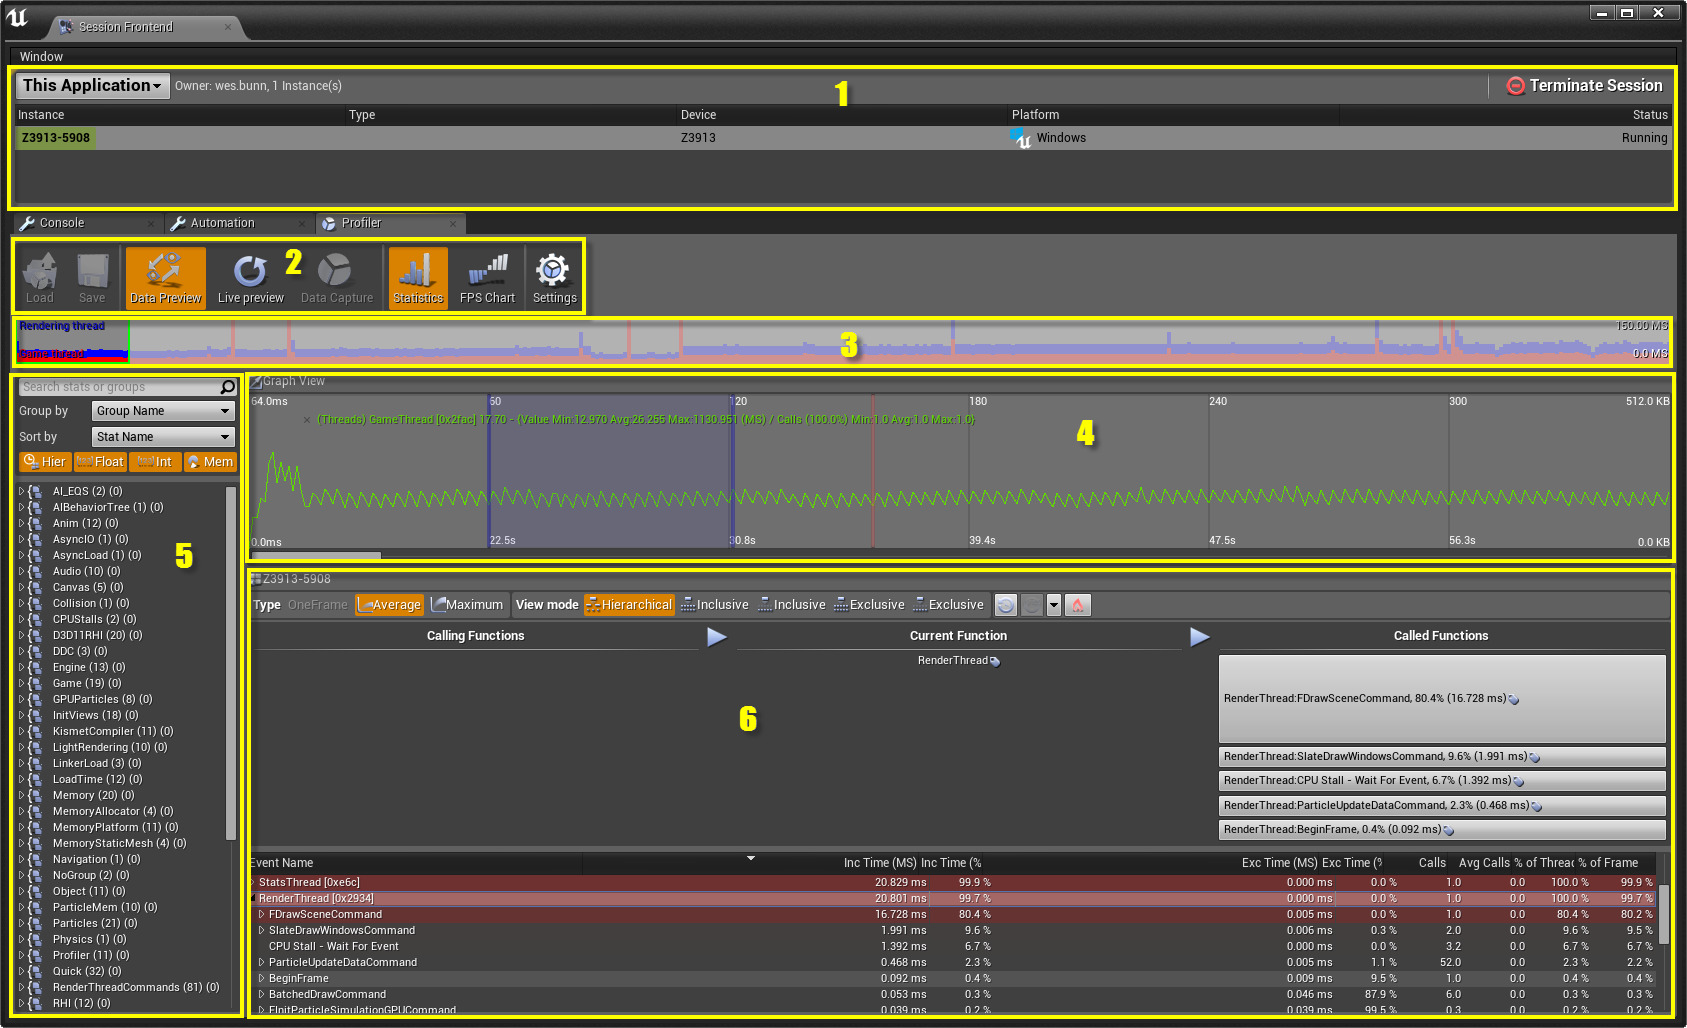
\includegraphics[width=\paperwidth, height=\paperheight]
            {unreal_profiler.jpg}}
          \begin{frame}
          \end{frame}
          }

          \frametitle{Nvidia nsight}
          {
            \setbeamercolor{footline}{fg=white}
            \usebackgroundtemplate{
              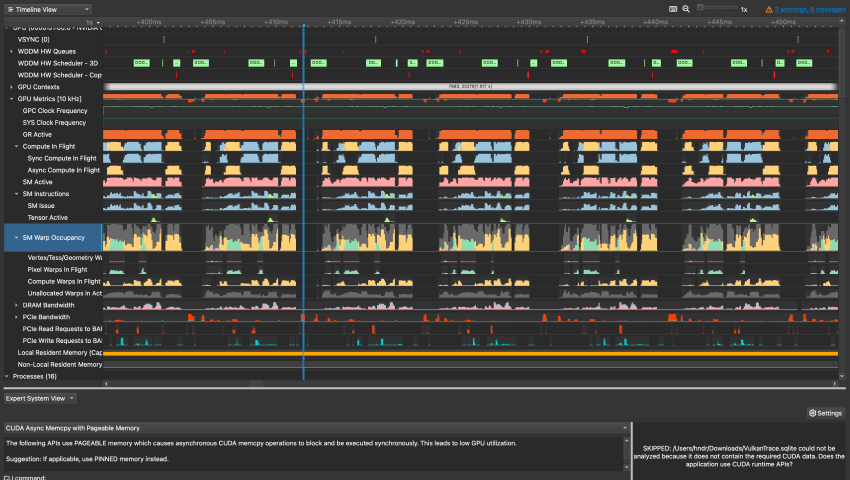
\includegraphics[width=\paperwidth, height=\paperheight]
              {nvida_nsighty.jpg}}
            \begin{frame}
            \end{frame}
            }
          

          \begin{frame}
          \frametitle{Nsight - Analiza FPS}
          \center
          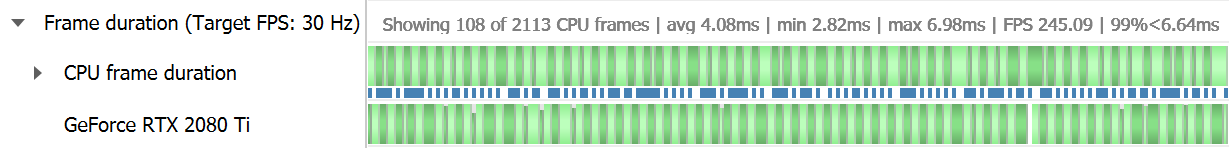
\includegraphics[width=1\textwidth]{fps_overview.png}
          % Ile klatek pokazaliśmy na ile
          % ile trwała średnio klatka
          % Ile trwała najkrótsza klatka
          % Ile trwała najdłuższa klatka
          % Przeciętne klatki na sekundę dla pokazanego wycinka
          % Tyle lub mniej czasu trwało 99% klatek
          \end{frame}

          \begin{frame}
            \frametitle{Nsight - Analiza FPS}
            \center
            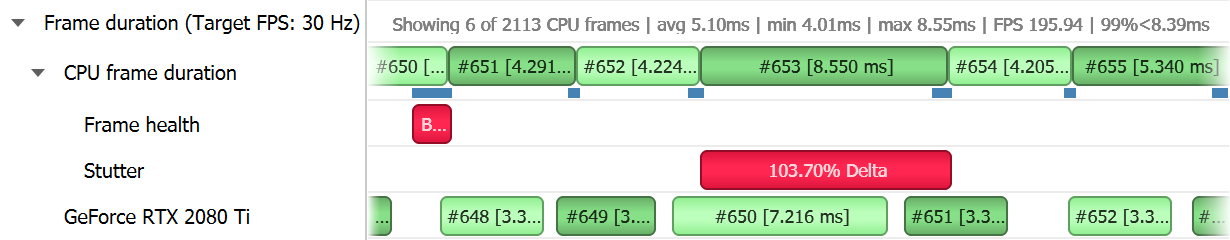
\includegraphics[width=1\textwidth]{stutter_row.png}
            % Wykrywanie "zawieszek"
            % Wykrywamy klatki których długość 
            % jest znacznie dłuższa od długości mediany pobliskich 19 klatek
            % zawieszka musi być dłuższa niż 4 milisekundy
            \end{frame}

            \begin{frame}
              \frametitle{Nsight - Analiza FPS}
              \center
                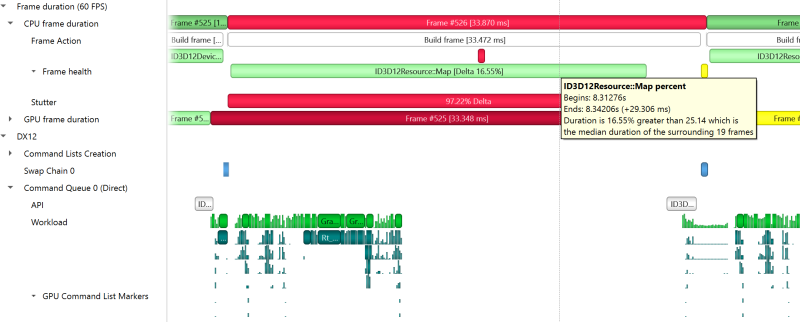
\includegraphics[width=1\textwidth]{dx12_frame_health.png}
                % Możemy sprawdzić jaka klatka miała zawieszkę
                % I jaka metoda w api tę zawieszkę spowodowała 
                \end{frame}
        
        \begin{frame}
          \frametitle{Nsight - Zużycie VRAM}
          \center
            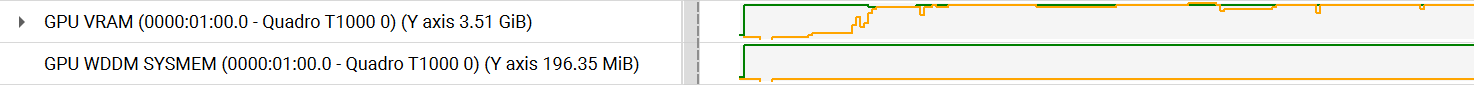
\includegraphics[width=1\textwidth]{memory_utilization.png}
            % Zielony -> ile pamięci mamy dostępnej
            % Pomarańczowy -> ile pamięci zużyliśmy 
            \end{frame}

            \begin{frame}
              \frametitle{Nsight - Zużycie VRAM}
              \center
                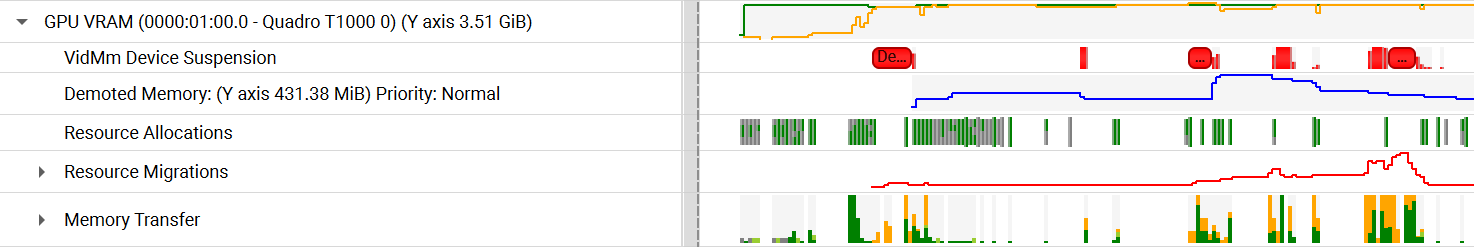
\includegraphics[width=1\textwidth]{memory_utilization_gpu_vram.png}
                % VidMm Device Suspension -> okresy czasku kiedy przetransferowano
                % Jeden duży zasób pamięci
                % Demoted Memory -> w GPU mamy local memory (szybsze) i global memory
                % (wolniejsze) to może nam mówić o "wyciekach" pamięci
                % źle zooptymalizowanej pamięci itd.
                % Allokacja pamięci -> zielone aplikacja, szare -> system
                \end{frame}

      \begin{frame}
        \frametitle{Nsight - Zużycie VRAM}
        \center
          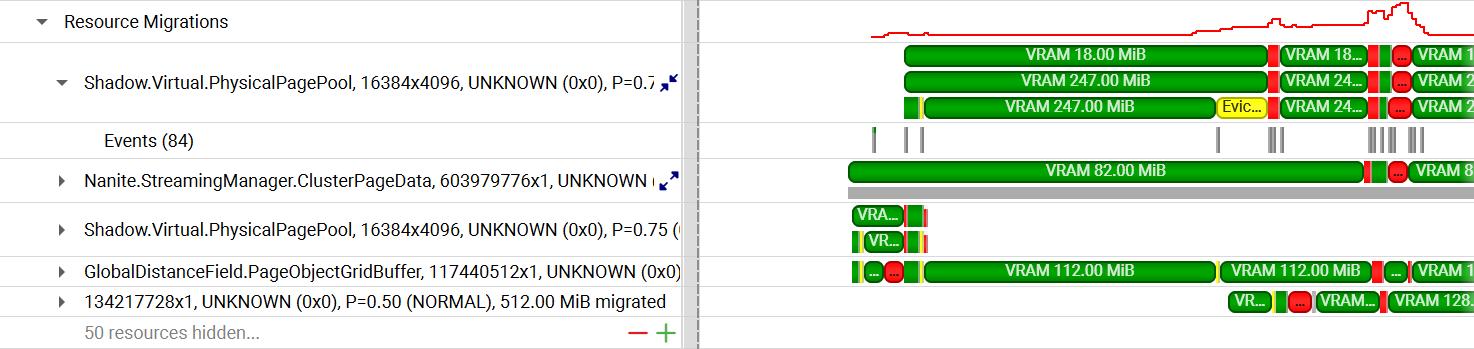
\includegraphics[width=1\textwidth]{memory_utilization_resource_migrations.png}
          % W kolejności co najwięcej zużyło zasobów
          % Konkretnie ile i kiedy
          \end{frame}

          \begin{frame}
            \frametitle{Nsight - Zużycie VRAM}
            \center
              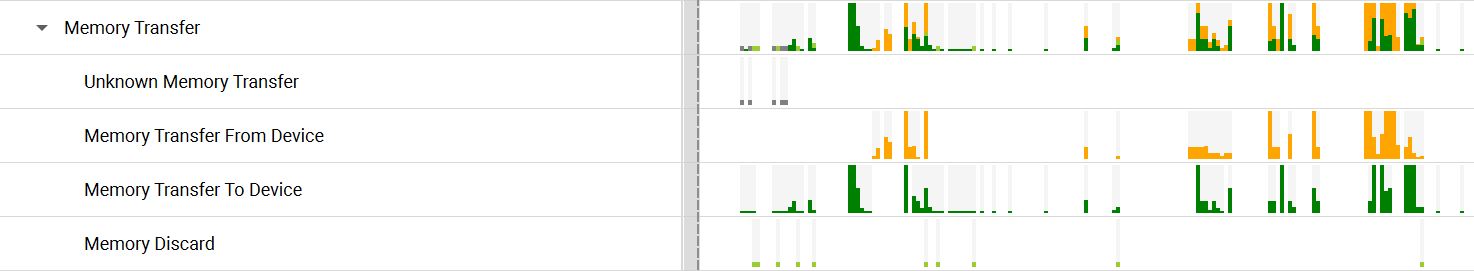
\includegraphics[width=1\textwidth]{memory_utilization_memory_transfer.png}
              % W kolejności co najwięcej zużyło zasobów
              % Konkretnie ile i kiedy
              \end{frame}

        \begin{frame}
        \frametitle{Jak porównywać?}
        \begin{itemize}
          \item Stworzenie gry na obu
          \item Porównywanie istniejących gier 
          \item Porównanie samych edytorów 
        \end{itemize} 
        \end{frame}

        {
          \setbeamercolor{footline}{fg=white}
          \usebackgroundtemplate{
            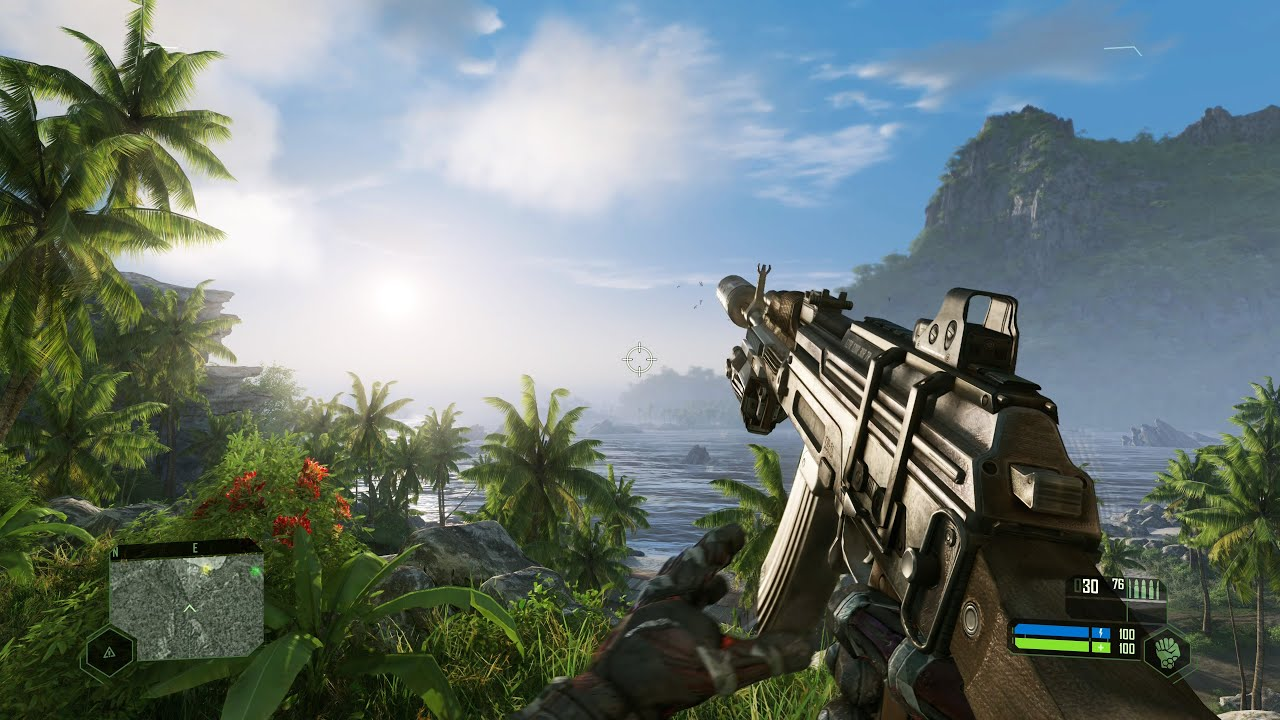
\includegraphics[width=\paperwidth, height=\paperheight]
            {maxresdefault (1).jpg}}
          \begin{frame}
          \end{frame}
          }

        \begin{frame}
          \frametitle{Wybór gatunku} 
          FPS: 
            \begin{itemize}
              \item Wystarczająco skomplikowany
              \item Grafika
              \item Fizyka
              \item Klasyczny benchmark 
              % Wolfenstein, Doom, Quake, Crysis
            \end{itemize}
        \end{frame}
        \begin{frame}
          \frametitle{Problem}
          Inklinacja Silnika \\ 
          \begin{itemize} 
          \item $ \frac{2478}{39713} \approx 6\%  $ gier Unity to FPS \\ 
          \item  $ \frac{1765}{11158} \approx 15\% $ gier Unreal to FPS \\ 
          \end{itemize}
        Źródło: steamdb.info
        \end{frame}

        \begin{frame}
          \frametitle{Wybór gatunku} 
          Bullet hell: 
            \begin{itemize}
              \item Wystarczająco skomplikowany 
              \item Grafika
              \item Czas jest ważny 
              % W Bullet hell czas jest ważny, gra musi być płynna
            \end{itemize}
        \end{frame}

        {
          \setbeamercolor{footline}{fg=white}
          \usebackgroundtemplate{
            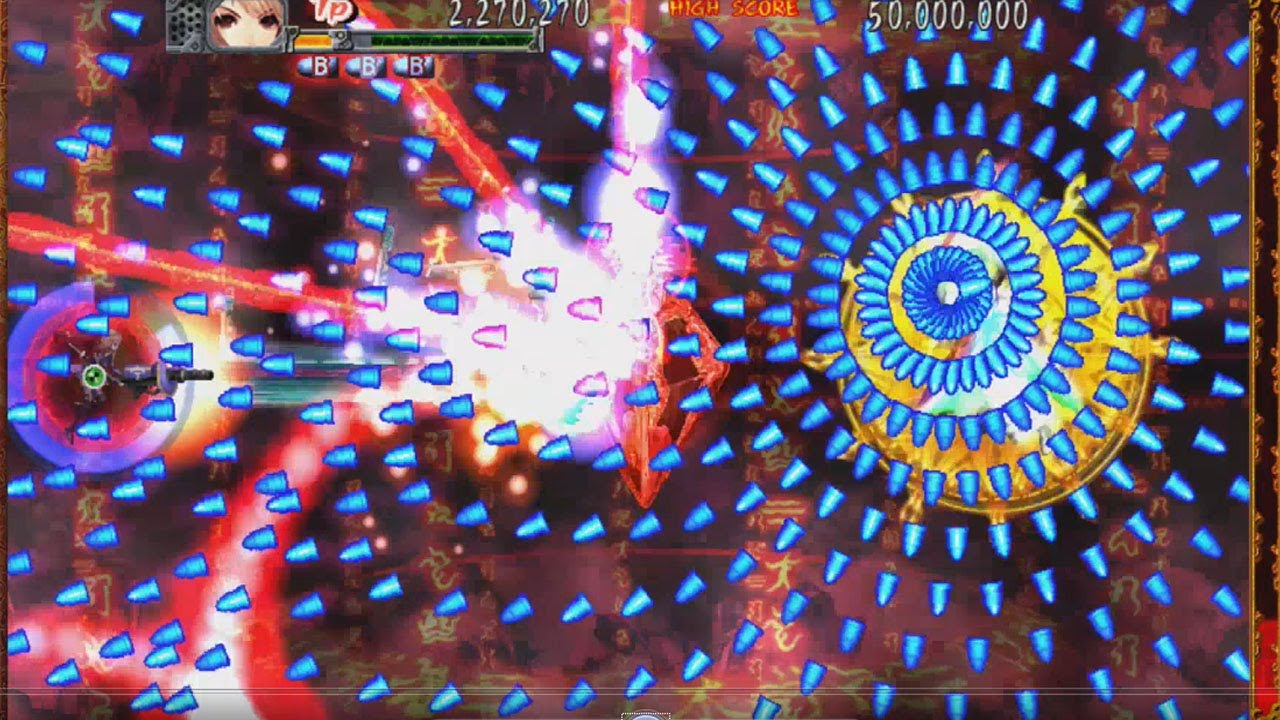
\includegraphics[width=\paperwidth, height=\paperheight]
            {maxresdefault.jpg}}
          \begin{frame}
          \end{frame}
          }
        \begin{frame}
          \frametitle{Wyzwania}
          \begin{itemize}
            \item Sprzęt 
            % Ten sam, jeden i ten sam komputer użyty w procesie kreacji obu
            \item Umiejętności 
            % Nie mam 
            \item Podobne wersje silnika 
            % Użyje ostatniego LTS
            \item Inklinacja Silnika \\ (3\% Unity, 2.4\% Unreal) 
            % ??? Ch 
            % 1577 FPS UNITY, 271 FPS UNREAL
            % 39713 Total Unity, 11158 Total Unreal (proporcjonalnie 2 razy więcej :<)
          \end{itemize}  
        \end{frame}  

      \begin{frame} 
        \frametitle{Ocena łatwości użycia}
        \begin{itemize}
          \item Dokumentacja
          \item Intuicyjność
          \item Materiały 
          \item Zasoby (Assety)  
          \item Dostępne funkcje
        \end{itemize}
      \end{frame}



      \begin{frame} 
        \frametitle{Po stworzeniu}
        Przejść obie gry, monitorując używając Nvidia Nsight i porównać wyniki
      \end{frame}


    \section{Źródła}
\begin{frame}
  \frametitle{Źródła}
    \begin{itemize}
        \item \href{https://steamdb.info/}{https://steamdb.info/}
    \item \href{https://docs.nvidia.com/nsight-systems}{https://docs.nvidia.com/nsight-systems}
    \item An Overview Study of Game Engines, Faizi Noor Ahmad 
    \item Game Engine Architecture, Jason Gregory
    \end{itemize}
    \end{frame}

\end{document}